\documentclass{HSEtitle}
\usepackage{lipsum}
\usepackage{mathtools}

\def\multiset#1#2{\ensuremath{\left(\kern-.3em\left(\genfrac{}{}{0pt}{}{#1}{#2}\right)\kern-.3em\right)}}


\everymath{\displaystyle}
%%%%%%%%%%%%%%%%%%%%%%%%%%%%%%%%
%%% ТЕКСТ РАБОТЫ %%%%%%%%%%%%%%%
\begin{document}

Подготовили Шевцов Лев и Дильдин Илья ПАДИИ

\section{Пункт 1}

Для проведения эксперемента фиксировалась выборка размером 100, k равное 5 и d равное 0.2. $\alpha$ варьировалась от 0.5 до 10 с делением на 60 значений. Усреднение шло по 10 различным значениям, так как такое уже позволило понять форму большенства распределений. 


\begin{figure}[hb]
    \centering
    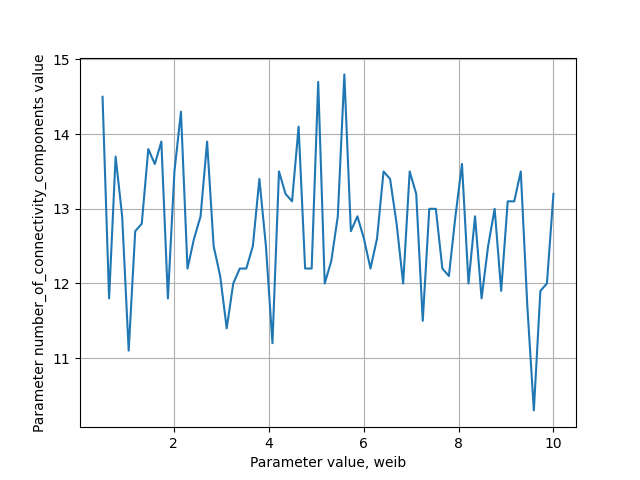
\includegraphics[width=0.65\linewidth]{weib_alpha_knn.png}
    \caption{Зависимость числа компонент связности от $\alpha$ при распределении weibull}
    \label{fig:enter-label}
\end{figure}

В случае анализа числа компонент связности в knn при обоих распределениях (рис. 1 и рис. 2) их распределение судя по всему независимо от $\alpha$ и имеет при наших условиях среднее около 12.5 в случае weibull и 11 в случае с exp.

\pagebreak

\begin{figure}[h]
    \centering
    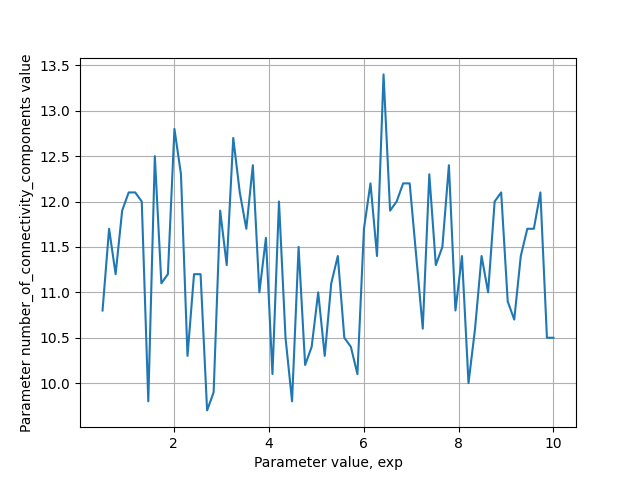
\includegraphics[width=0.65\linewidth]{exp_alpha_knn.png}
    \caption{Зависимость числа компонент связности от $\alpha$ при распределении exp}
    \label{fig:enter-label}
\end{figure}

\begin{figure}[h]
    \centering
    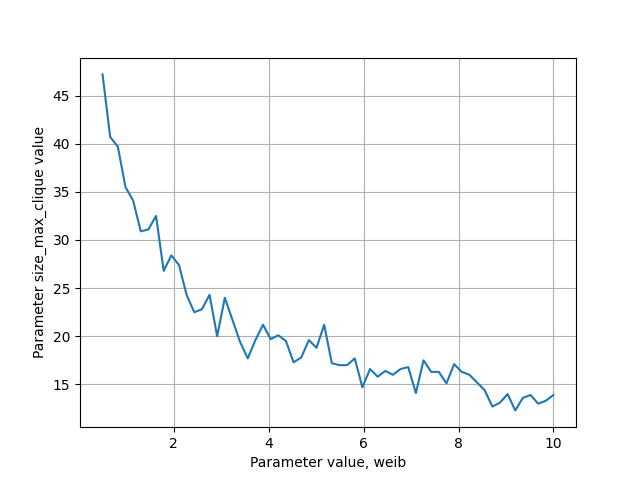
\includegraphics[width=0.65\linewidth]{weib_alpha.png}
    \caption{Зависимость максимальной клики от $\alpha$ при распределении weibull}
    \label{fig:enter-label}
\end{figure}

\pagebreak

\begin{figure}[ht]
    \centering
    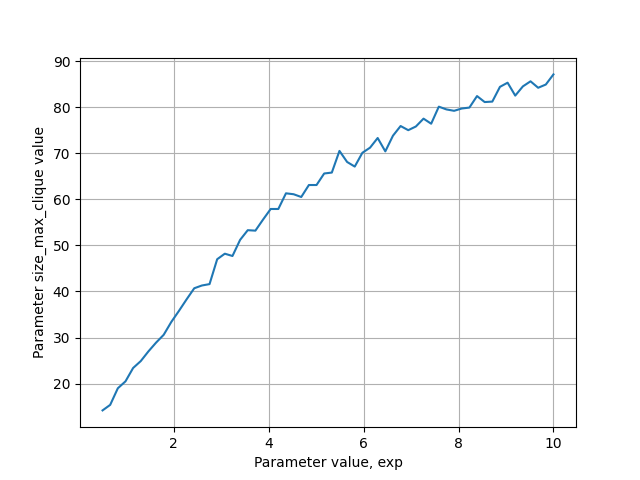
\includegraphics[width=0.65\linewidth]{exp_alpha.png}
    \caption{Зависимость максимальной клики от $\alpha$ при распределении exp}
    \label{fig:enter-label}
\end{figure}

В случае же с максимальной кликой видно (рис. 3 и рис. 4), что распределение напоминает степенну функцию, но с совершенно разными степенями. По моим рассчетам при наших условиях степень составляет около  в случае weibull и 2/5 в случае с exp.

\begin{figure}[hb]
    \centering
    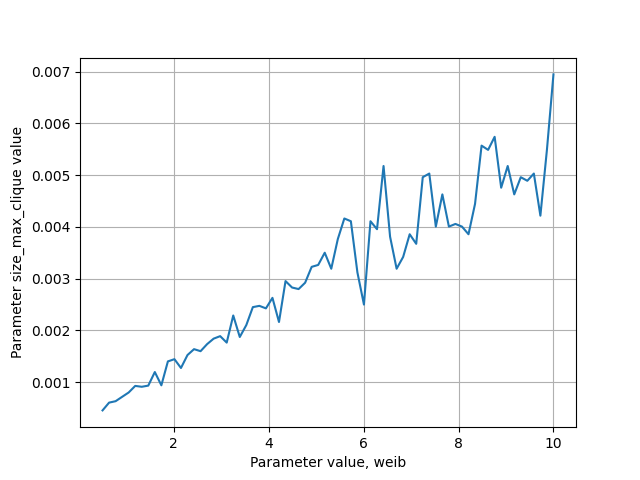
\includegraphics[width=0.65\linewidth]{weib_alpha_fix.png}
    \caption{Зависимость максимальной клики от $\alpha$ при распределении weibull после выравнивание возведением в степень}
    \label{fig:enter-label}
\end{figure}

\begin{figure}
    \centering
    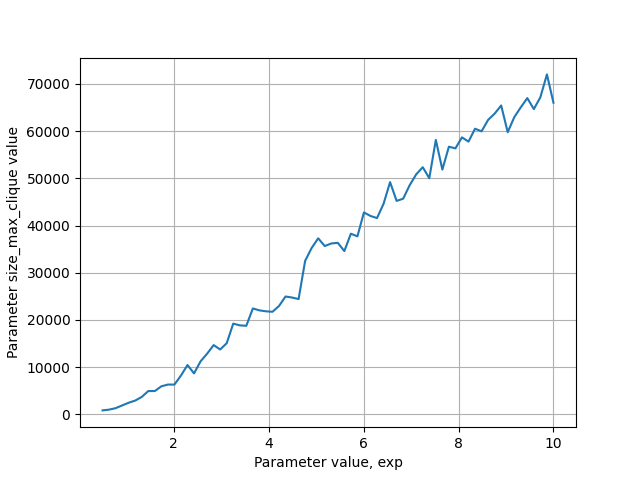
\includegraphics[width=0.65\linewidth]{exp_alpha_fix.png}
    \caption{Зависимость максимальной клики от $\alpha$ при распределении exp после выравнивание возведением в степень}
    \label{fig:enter-label}
\end{figure}

\pagebreak

\section{Пункт 2}

Для проведения эксперемента фиксировалась данное в задании $\alpha$ и значения k проходили от 2 до 20 с шагом 1, значения d проходили от 0.05 до 10 с делением на 60 участков и значения n проходили от 50 до 100 с шагом 2. Усреднение шло по 10 различным значениям аналогично первому пункту.

Тут можно отметить, что от k зависимость степенная с отрицательным коэффициентом в обоих случаях, от d зависимость степенная с коэффициентом меньше 0, а от n зависимость линейная положительная во всех случаях, при том с меньшей дисперсией при подсчете кликового числа.

\section{Пункт 3}

После запуска функции мощность полученного А на выборке размером 300 и с количеством итераций 1000 составило power =  0.9919999999999998, error =  0.9999999999999998 для knn и power = 0.5780000000000001, error =  1.0 для dist. Это говорит о том, что в случае с числом компонент связности принимаемые значения похожи друг на друга и обоих плотностей, а вот кликовое число достаточно разнится, но все равно вероятность ошибится можно оценить примерно как 50 на 50.

\begin{figure}[hb]
    \centering
    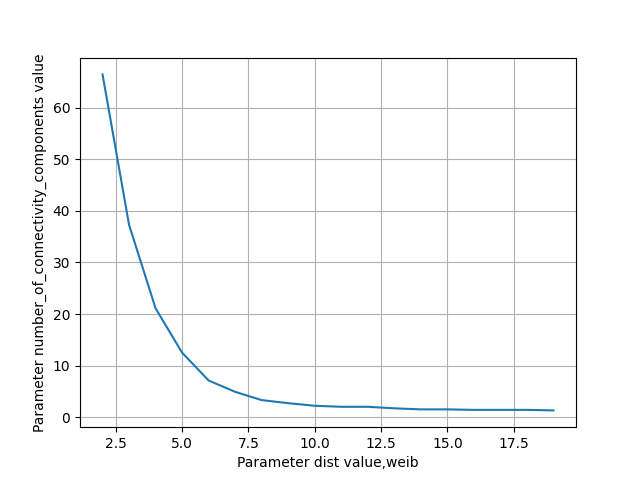
\includegraphics[width=0.65\linewidth]{weib_k.png}
    \caption{Зависимость числа компонент связности от k при распределении weibull}
    \label{fig:enter-label}
\end{figure}

\begin{figure}[h]
    \centering
    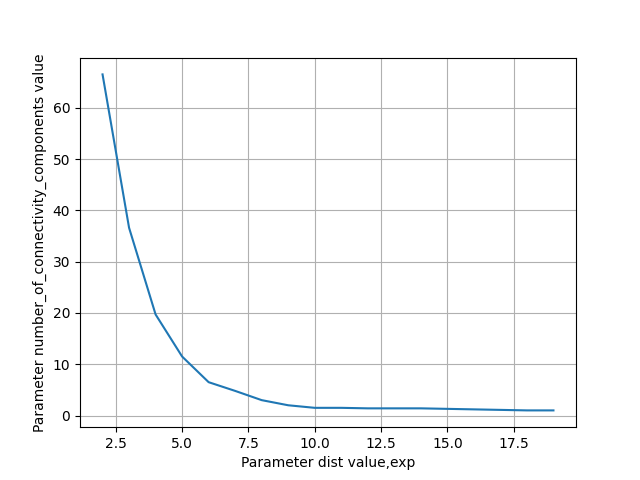
\includegraphics[width=0.65\linewidth]{exp_k.png}
    \caption{Зависимость числа компонент связности от k при распределении exp}
    \label{fig:enter-label}
\end{figure}

\begin{figure}[h]
    \centering
    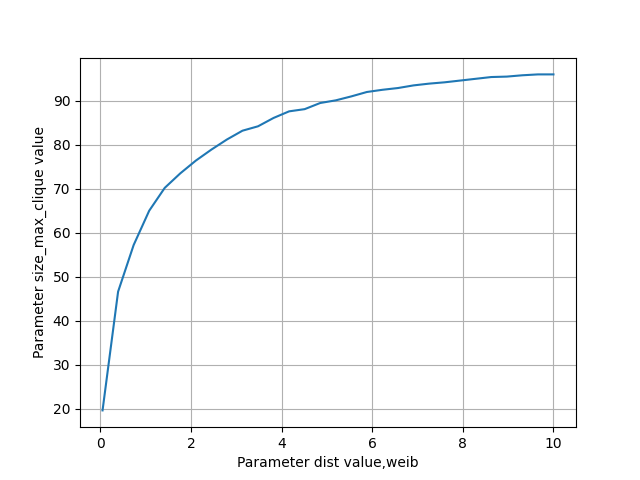
\includegraphics[width=0.65\linewidth]{weib_d.png}
    \caption{Зависимость размера максимальной клики от d при распределении weibull}
    \label{fig:enter-label}
\end{figure}

\begin{figure}[h]
    \centering
    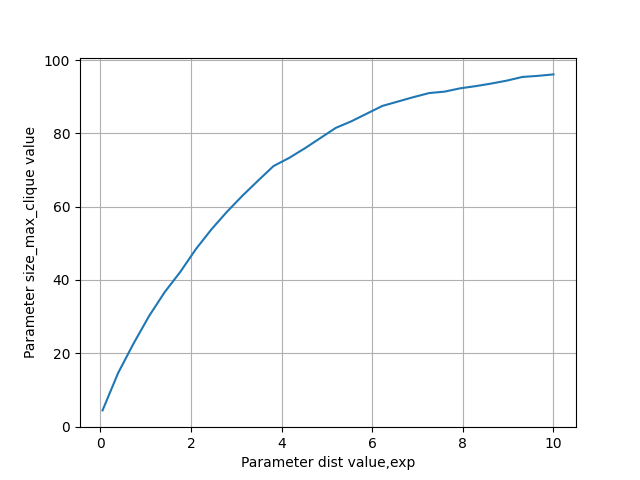
\includegraphics[width=0.65\linewidth]{exp_d.png}
    \caption{Зависимость размера максимальной клики от d при распределении exp}
    \label{fig:enter-label}
\end{figure}

\begin{figure}[h]
    \centering
    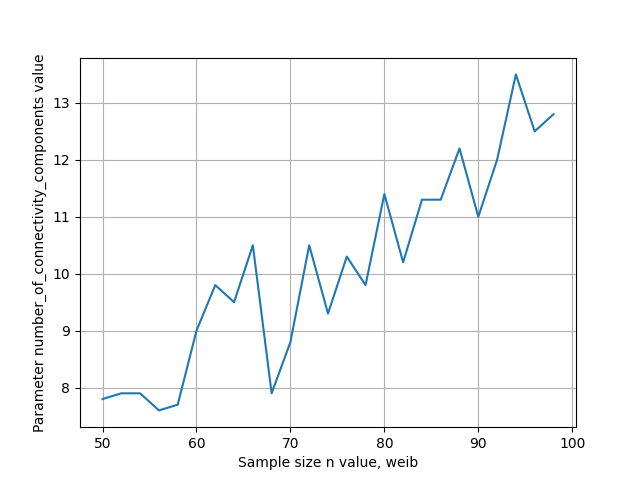
\includegraphics[width=0.65\linewidth]{weib_n_knn.png}
    \caption{Зависимость числа компонент связности n при распределении weibull}
    \label{fig:enter-label}
\end{figure}

\begin{figure}[h]
    \centering
    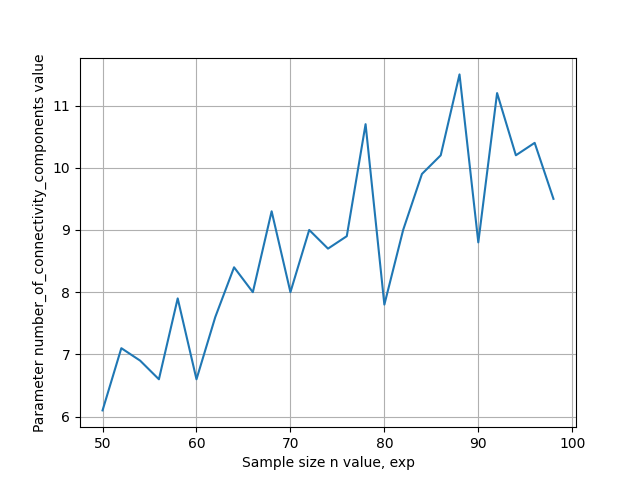
\includegraphics[width=0.65\linewidth]{exp_n_knn.png}
    \caption{Зависимость числа компонент связности n при распределении exp}
    \label{fig:enter-label}
\end{figure}

\begin{figure}[h]
    \centering
    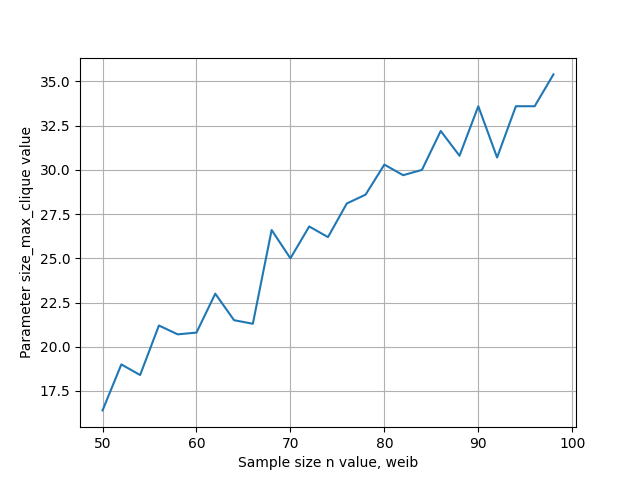
\includegraphics[width=0.65\linewidth]{weib_n.png}
    \caption{Зависимость размера максимальной клики от n при распределении weibull}
    \label{fig:enter-label}
\end{figure}

\begin{figure}[h]
    \centering
    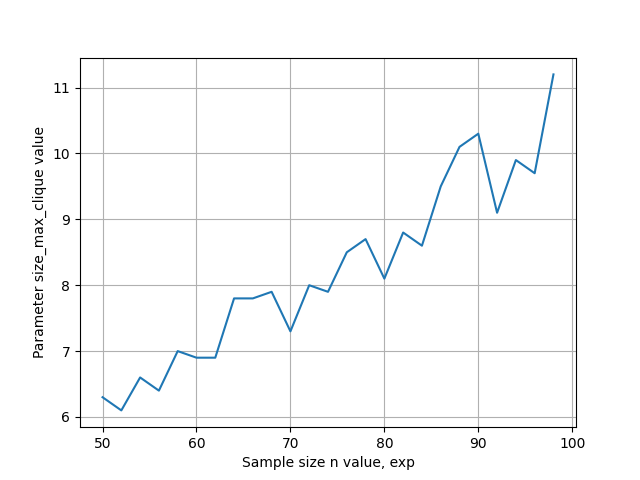
\includegraphics[width=0.65\linewidth]{exp_n.png}
    \caption{Зависимость размера максимальной клики от n при распределении exp}
    \label{fig:enter-label}
\end{figure}


\section{Анализ функций по их параметрам}

Для проведения экспериментов фиксировалась выборка размера размера 100, k равное 5 и d равное 0.2:

1)stud распеределение(рис 15)  

Максимальная степень графа не влияет на числовую характеристику при изменении параметра 
\begin{figure}
    \centering
    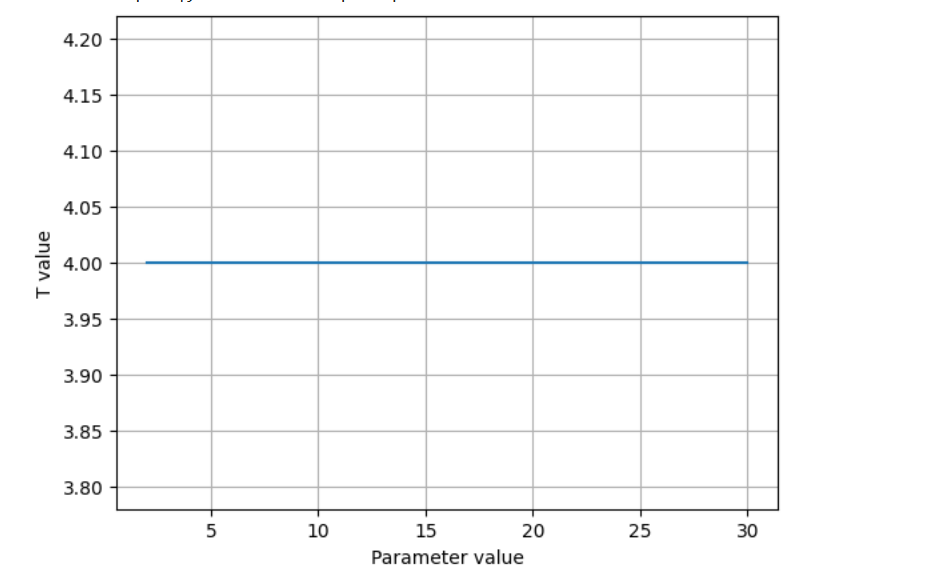
\includegraphics[width=0.5\linewidth]{11.png}
    \caption{Анализ по параметрам - stud распеределение}
    \label{fig:enter-label}
\end{figure}

2)lap распеределение(рис 16)  

Размер максимального независимого множества к числовой характеристике стремиться к прямой зависимости, то есть чем больше параметр тем больше размер максимального независимого множества
\begin{figure}
    \centering
    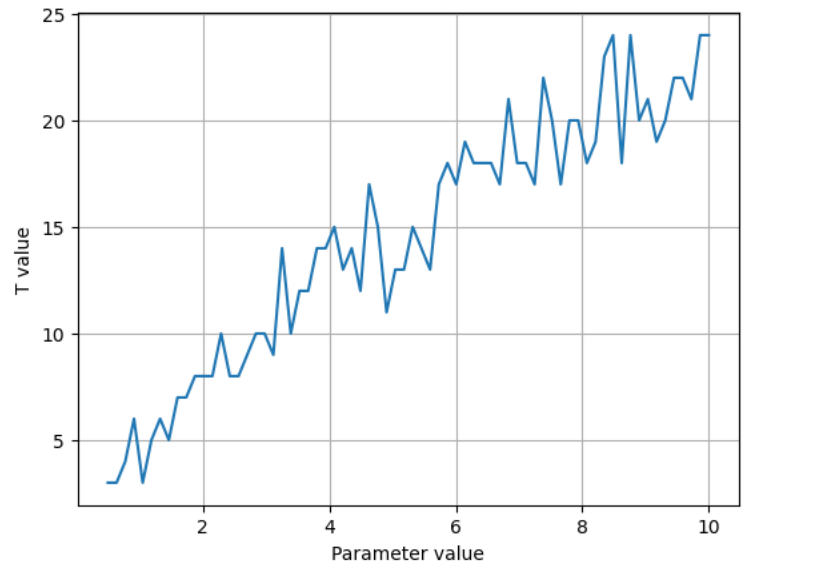
\includegraphics[width=0.5\linewidth]{12.png}
    \caption{Анализ по параметрам - lap распеределение}
    \label{fig:enter-label}
\end{figure}



\section{Анализ функций по k и d}

Для проведения экспериментов фиксировалась выборка размера размера 100:

1)stud распеределение(рис 17) 

Максимальная степень графа имеет линейную зависимость при изменении параметра k при создании gk
\begin{figure}
    \centering
    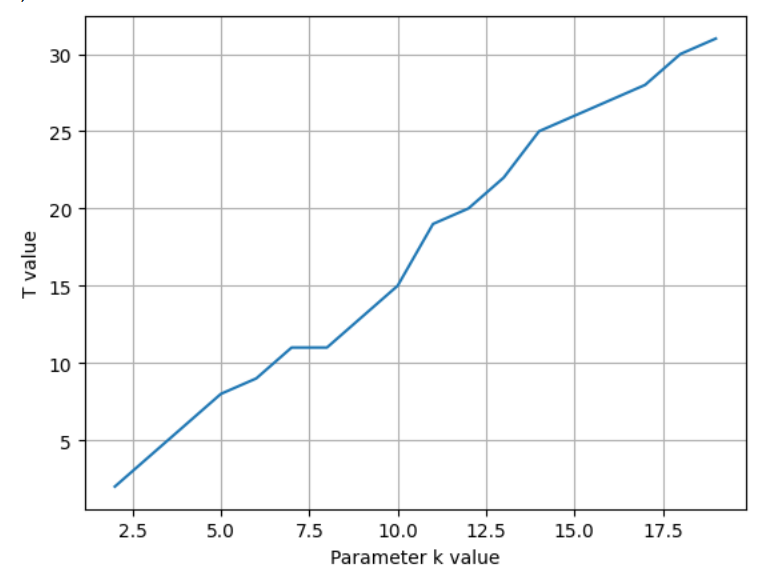
\includegraphics[width=0.5\linewidth]{15.png}
    \caption{Анализ по k  - stud распеределение}
    \label{fig:enter-label}
\end{figure}

2)lap распеределение(рис 18) 

Размер максимального независимого множества к d проявляет примерно обратную зависимость
\begin{figure}
    \centering
    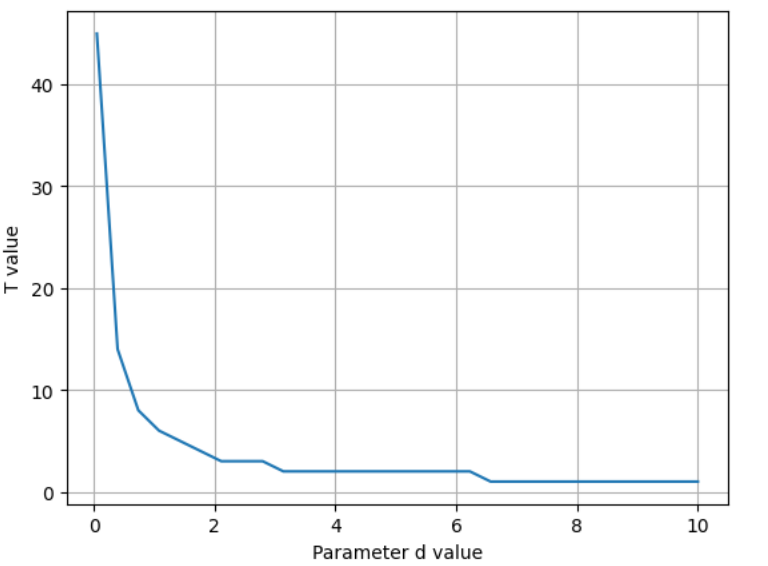
\includegraphics[width=0.5\linewidth]{17.png}
    \caption{Анализ по d - lap распеределение}
    \label{fig:enter-label}
\end{figure}



\section{Анализ функций по выборке n}

Для проведения экспериментов фиксировалась k равное 5 и d равное 0.2:

1)stud распеределение(рис 19)

Максимальная степень графа не влияет на числовую характеристику при изменении выборки
\begin{figure}
    \centering
    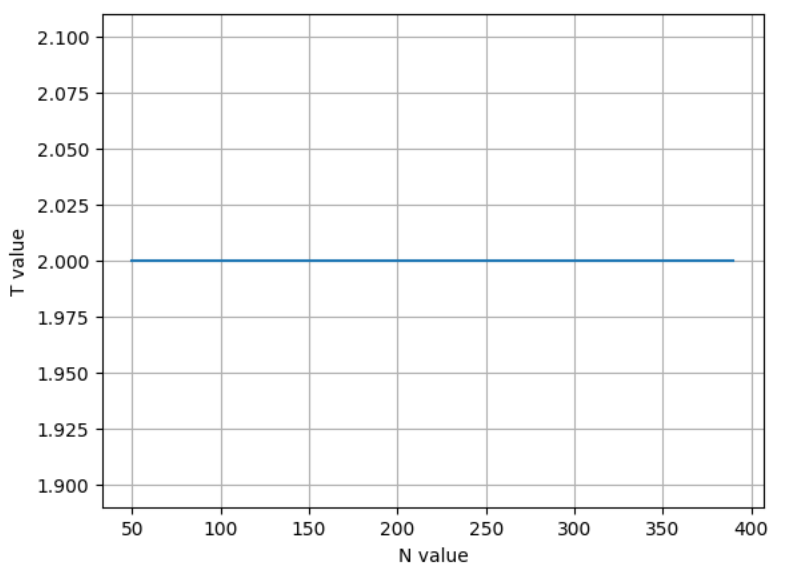
\includegraphics[width=0.5\linewidth]{6.png}
    \caption{Анализ по n - stud распеределение}
    \label{fig:enter-label}
\end{figure}

2)lap распеределение (рис 20)

Размер максимального независимого множества к размеру выборки n стремиться к прямой зависимости, то есть чем больше d тем больше размер максимального независимого множества
\begin{figure}
    \centering
    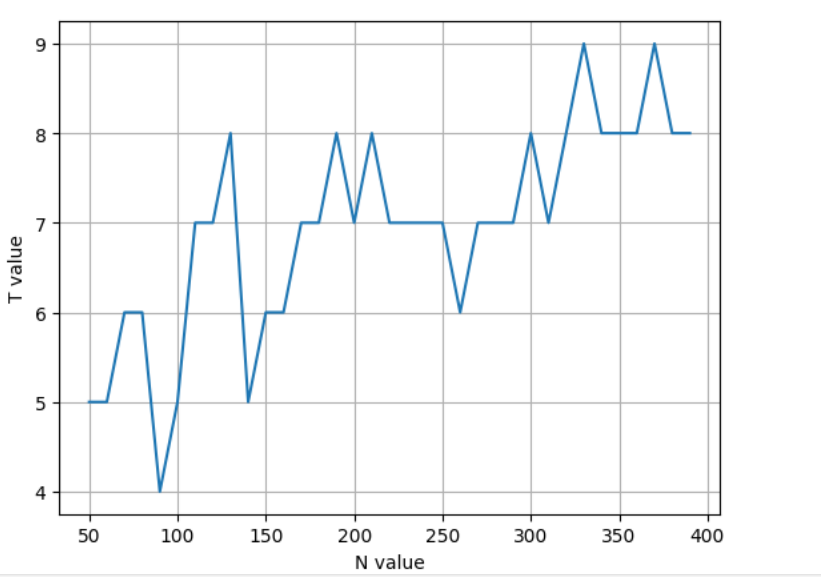
\includegraphics[width=0.5\linewidth]{8.png}
    \caption{Анализ по n - lap распеределение}
    \label{fig:enter-label}
\end{figure}



\section{Пункт 3}

Для Лапласа и Стьюденса:

После запуска функции при выборке 300 и количества итераций 1000 мощность А  вышла 0.13, а ошибка 1.0.  Вероятность неправильно принять Н1 составляет не более 13 процентов.

\section{Часть 2. Исследование важность характеристик}

Важность признаков у stud и lap при постоянном выбранном нами n:

\texttt{max\_degree}: 0.6129

\texttt{size\_max\_independent\_set}: 0.3871

Важность признаков у exp и weib при постоянном выбранном нами n:

\texttt{number\_of\_connectivity\_components}: 0.4483

\texttt{size\_max\_clique}: 0.5517

Посмотрим как выглядит график при различных n(рисунки 21 и 22):

\begin{figure}
    \centering
    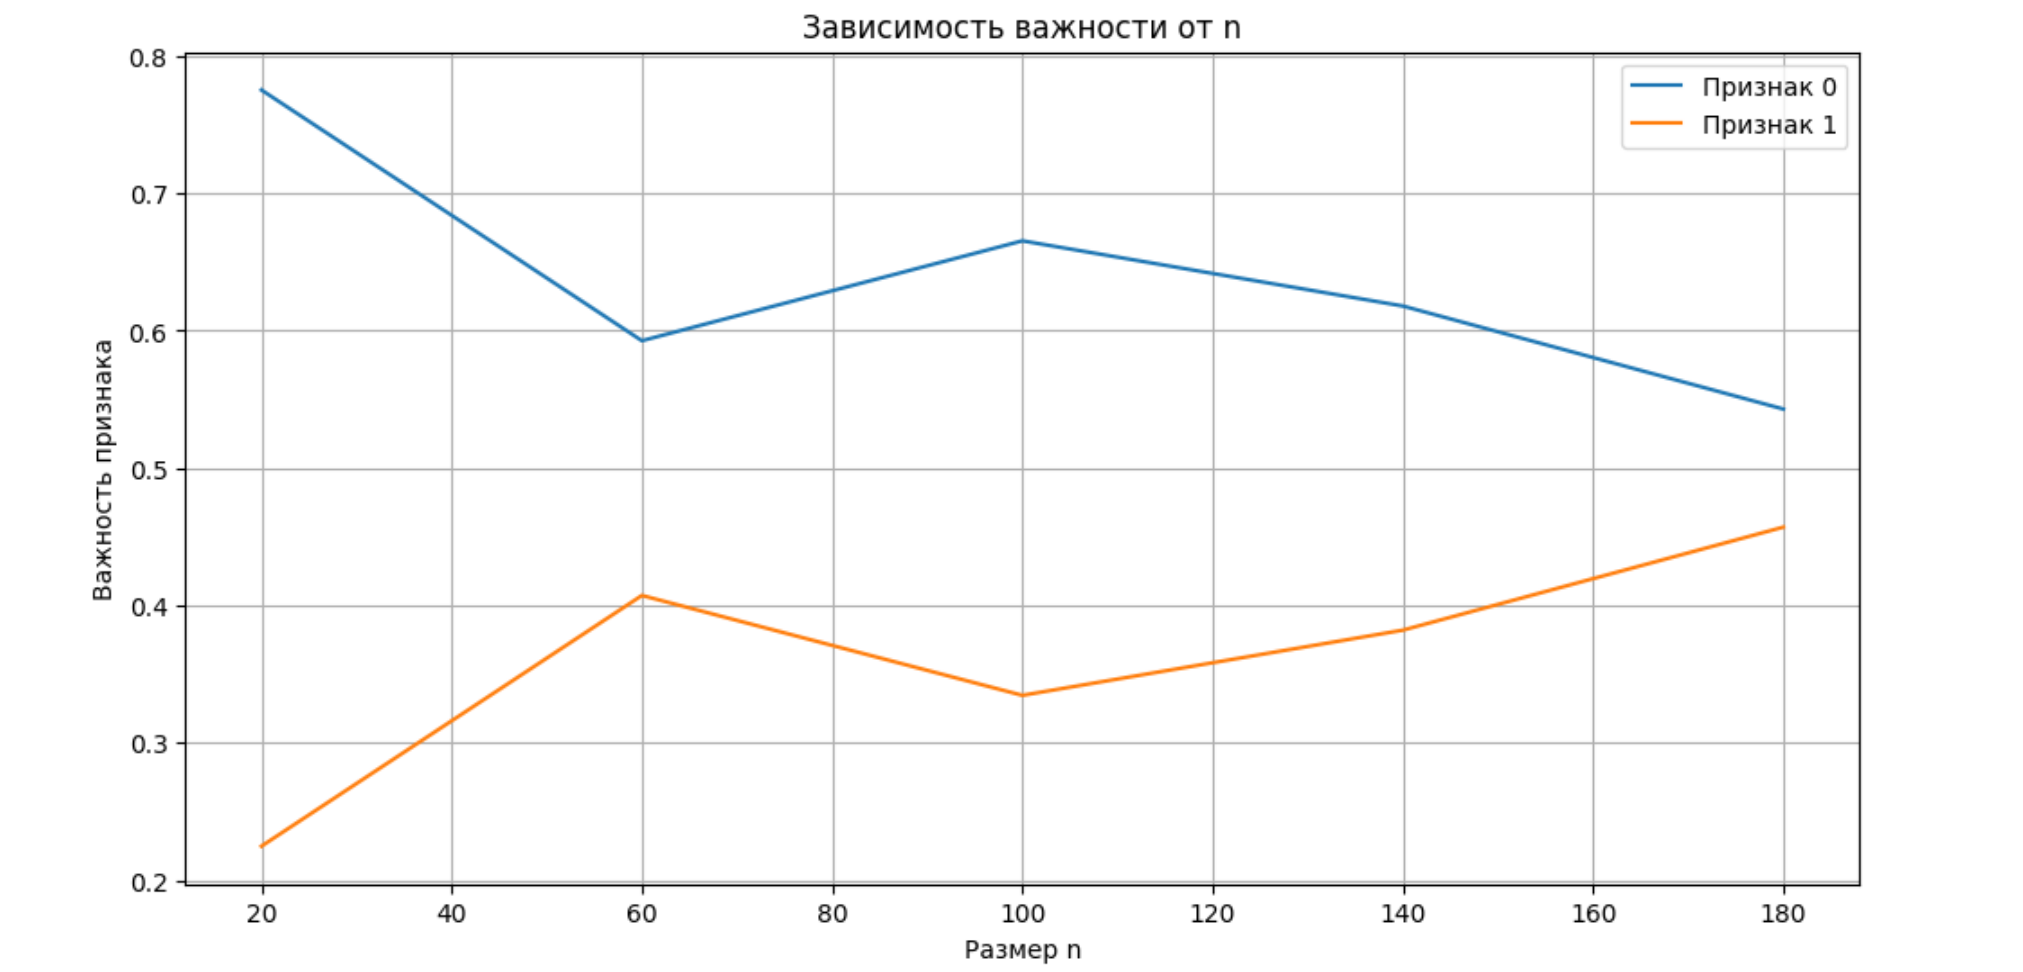
\includegraphics[width=0.5\linewidth]{importance1.png}
    \caption{Важность признаков у stud и lap}
    \label{fig:enter-label}
\end{figure}
\begin{figure}
    \centering
    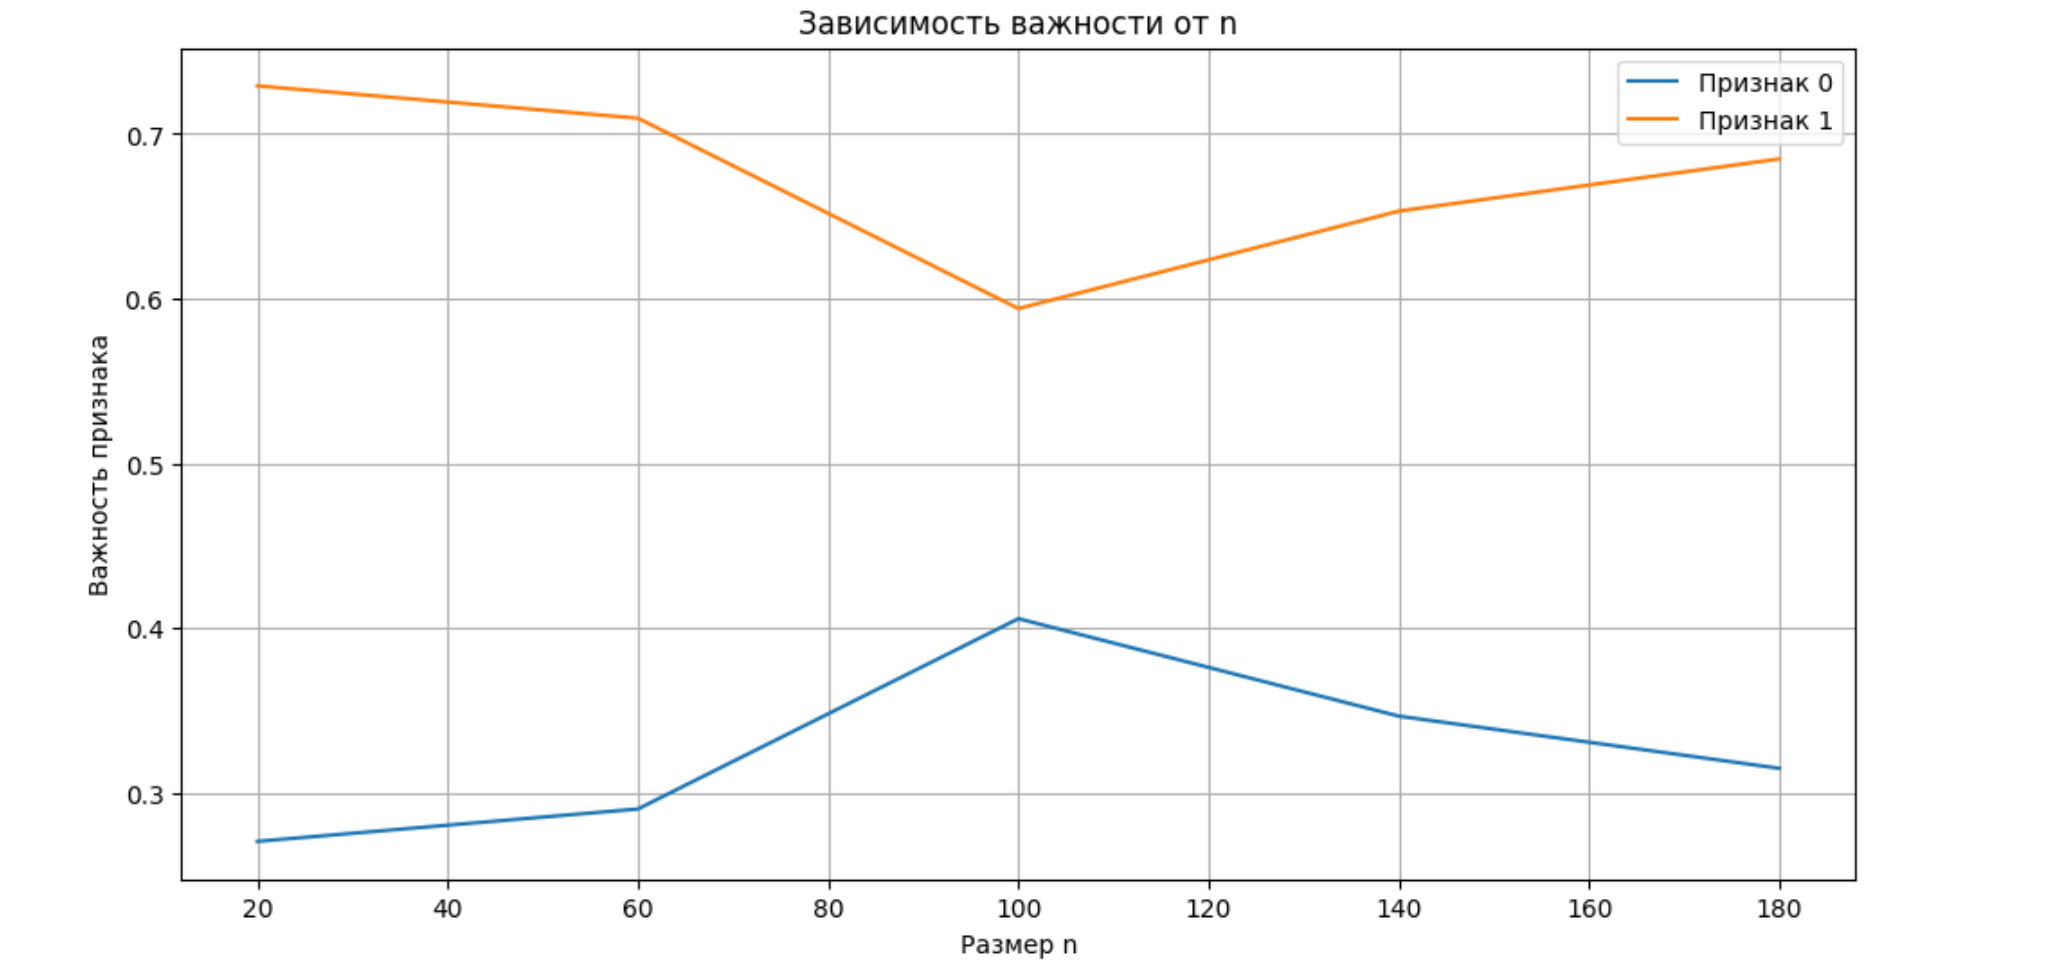
\includegraphics[width=0.5\linewidth]{importance2.png}
    \caption{Важность признаков у exp и weib}
    \label{fig:enter-label}
\end{figure}

Для stud и lap - синяя линия - \texttt{max\_degree}, а желтая  - \texttt{size\_max\_independent\_set}. Из этого можно сделать вывод, что для определения большую роль играет максимальная степень

Для exp и weib - синяя линия - \texttt{number\_of\_connectivity\_components}, а желтая  - \texttt{size\_max\_clique}. Из этого можно сделать вывод, что для определения большую роль играет число компонент связности.

\section{Часть 2. Исследование метрики}

Для stud и lap - при минимальном $n$ - лучшим алгоритмом будет K-ближайших соседей, при остальных n, чем больше n тем лучше результат, а при максимльном $n$ точность будет равна 1 для всех алгоритмов.

Также для каждого $n$ мы вывели Confusion matrix(рисунки 23-25)

Для exp и weib - при минимальном n - лучшим алгоритмом будет Логистическая регрессия и K-ближайших соседей, при остальных $n$, чем больше n тем лучше результат, а при максимльном $n$ Дерево и Логистическая регрессия будут лучшими алгоритмами.

Также для каждого $n$ мы вывели Confusion matrix(рисунки 26-28)

\section{Реализация}

В 1 части - каждый реализовывал свои функции

Создание gd - Лев, создание gk - Илья. Первый пункт - Лев и Илья, второй пункт - Лев и Илья, третий пункт - Илья.

Во 2 части - первый и второй пункт - Лев, третий - Илья.

\begin{figure}
    \centering
    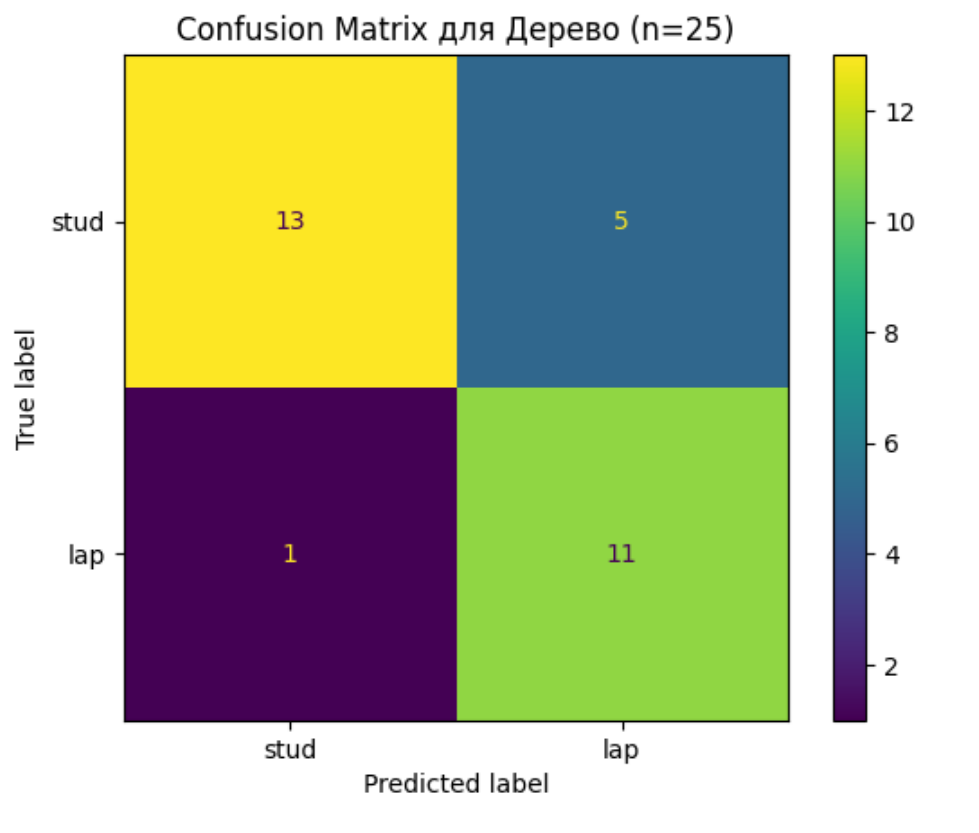
\includegraphics[width=0.5\linewidth]{Confusion matrix lap and stud 1.png}
    \caption{Confusion matrix lap and stud n=25}
    \label{fig:enter-label}
\end{figure}
\begin{figure}
    \centering
    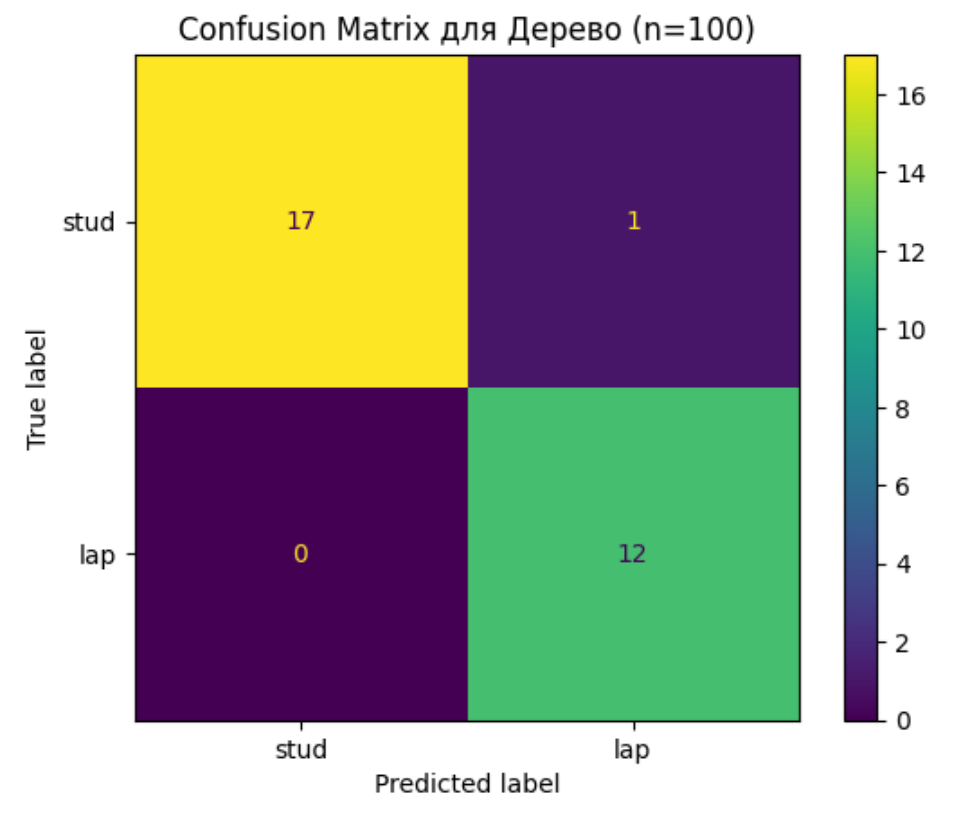
\includegraphics[width=0.5\linewidth]{Confusion matrix lap and stud 2.png}
    \caption{Confusion matrix lap and stud n=100}
    \label{fig:enter-label}
\end{figure}
\begin{figure}
    \centering
    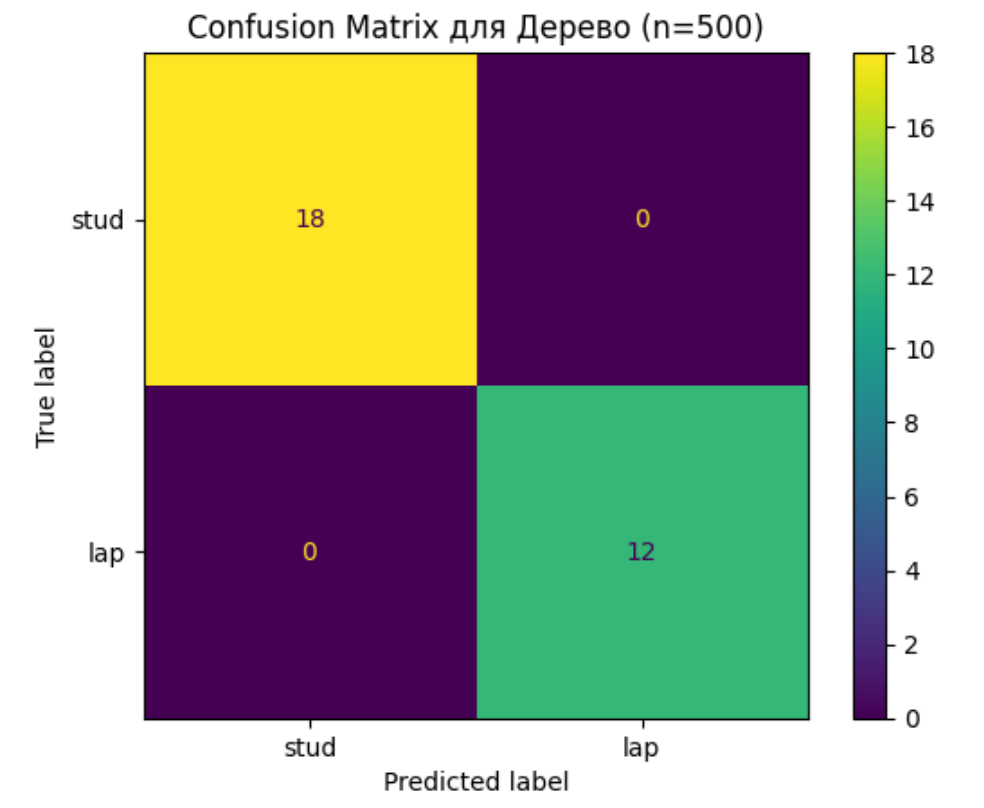
\includegraphics[width=0.5\linewidth]{Confusion matrix lap and stud 3.png}
    \caption{Confusion matrix lap and stud n=500}
    \label{fig:enter-label}
\end{figure}
\pagebreak
\begin{figure}
    \centering
    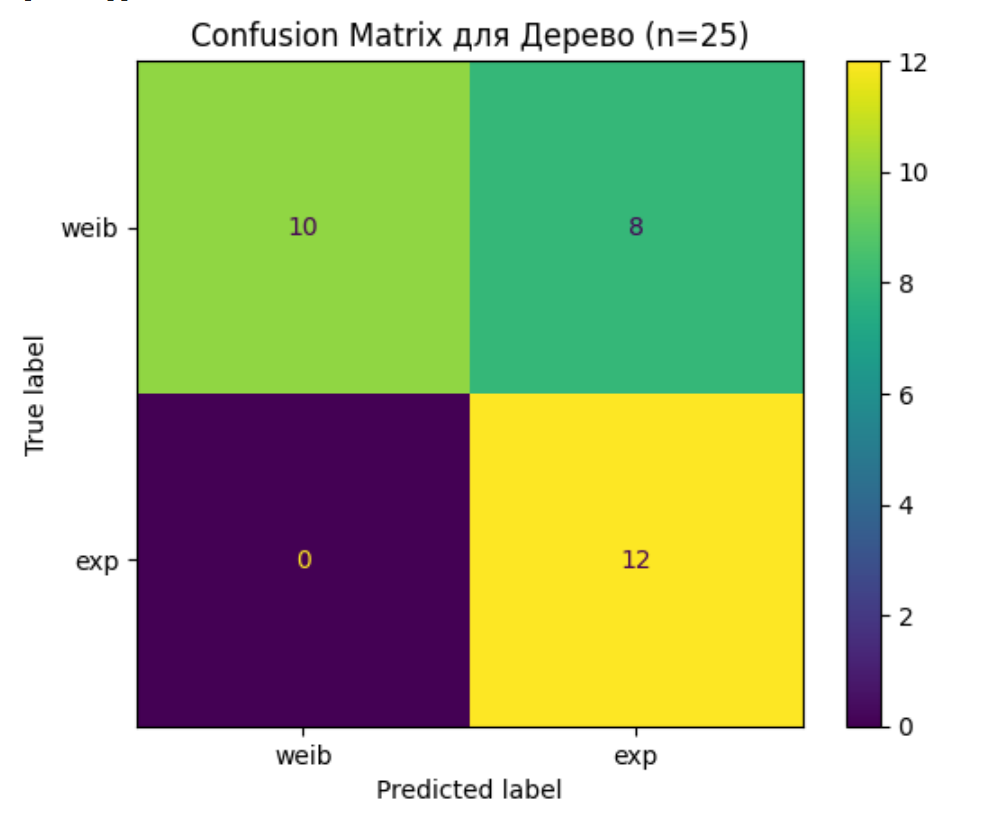
\includegraphics[width=0.5\linewidth]{Confusion matrix weih and exp 1.png}
    \caption{Confusion matrix weib and exp n=25}
    \label{fig:enter-label}
\end{figure}

\begin{figure}
    \centering
    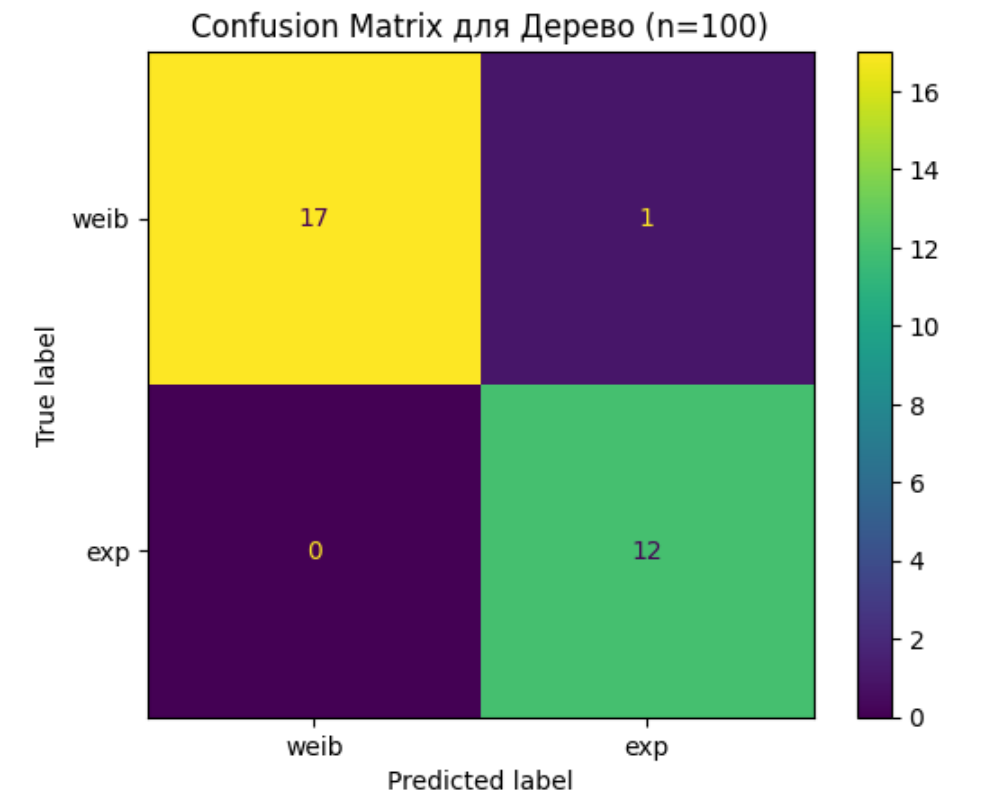
\includegraphics[width=0.5\linewidth]{Confusion matrix weih and exp 2.png}
    \caption{Confusion matrix weib and exp n=100}
    \label{fig:enter-label}
\end{figure}
\begin{figure}
    \centering
    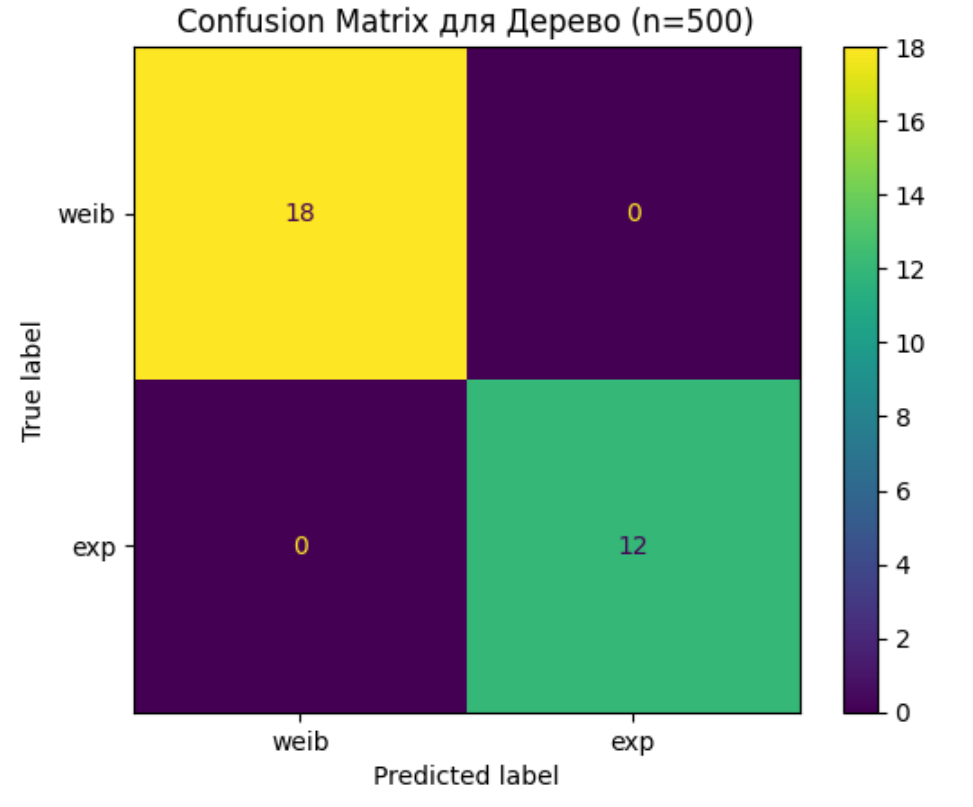
\includegraphics[width=0.5\linewidth]{Confusion matrix weih and exp 3.png}
    \caption{Confusion matrix weib and exp n=500}
    \label{fig:enter-label}
\end{figure}
\end{document}